\chapter{Prototyping Process}

The prototype did not begin as a polished scene. It moved through three practical layers: an early game concept in the one-pager \cite{onePager}, a narrowed architectural constraint document that removed non-essential systems \cite{architectureConstraints}, and a first-pass script list that defined the minimum compilable gameplay skeleton \cite{firstPassScripts}. WR2 records the point where these design decisions became a playable vertical slice. The narrative in this chapter follows the frozen WR2 snapshot rather than the team's longer-term target state, so partial and deferred items are kept explicit.

\section{Prototype}

Figure~\ref{fig:retrospective-wireframe} shows a retrospective low-fidelity wireframe rebuilt from the WR1 scope and the current scene layout. It is explicitly marked as retrospective because no separate low-fidelity mockup was archived in the local workspace before prototype implementation began. The wireframe is still useful in WR2 because it clarifies the intended information zones: turn state, hand controls, status feedback, and the board itself.

\begin{figure}[H]
\centering
\input{figures/retrospective-wireframe}
\caption{Retrospective low-fidelity wireframe reconstructed from WR1 scope and the current prototype layout}
\label{fig:retrospective-wireframe}
\end{figure}

The high-fidelity prototype evidence comes from the working Unity scene. Figure~\ref{fig:prototype-evidence} shows the current battle board and left-side battle UI, while Figure~\ref{fig:prototype-board} isolates the in-world battle scene used as the basis for interaction and screenshot capture.

\begin{figure}[H]
\centering
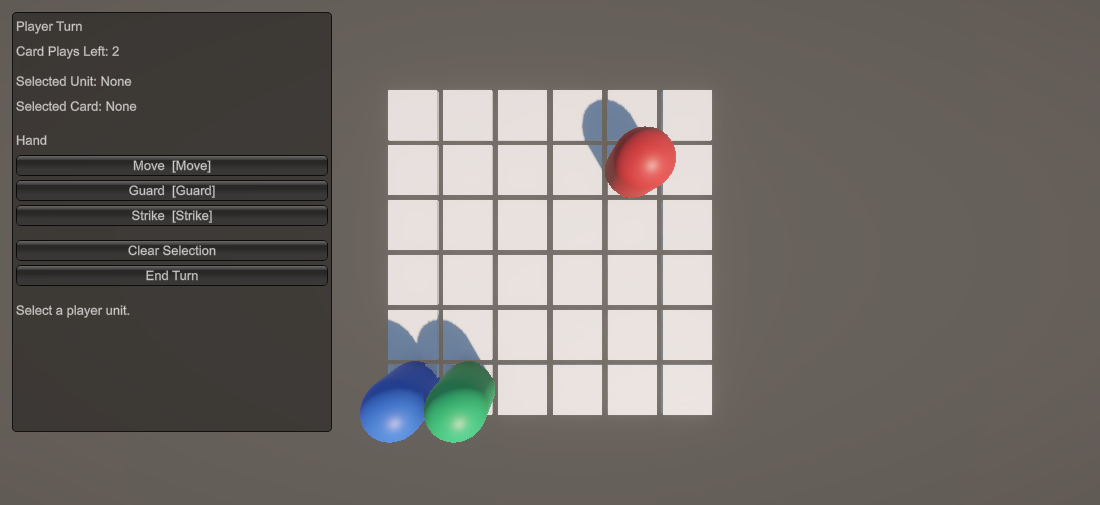
\includegraphics[width=0.88\textwidth]{media/battleui-play-check.png}
\caption{Current high-fidelity prototype with battle UI, starter hand, and 6x6 board}
\label{fig:prototype-evidence}
\end{figure}

\begin{figure}[H]
\centering
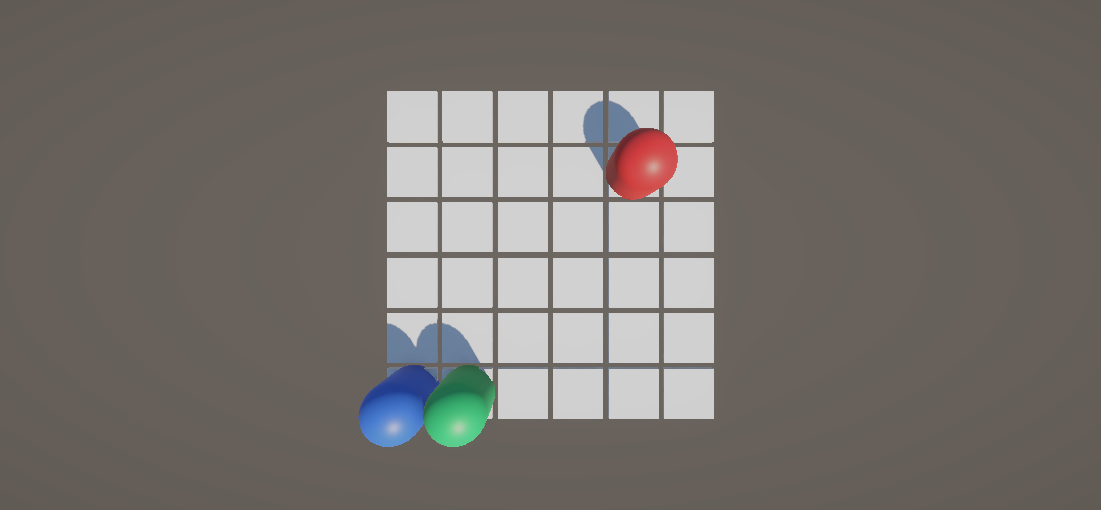
\includegraphics[width=0.88\textwidth]{media/tactical-cards-scene-inline.png}
\caption{Board-only view of the current playable battle scene}
\label{fig:prototype-board}
\end{figure}

The current frozen prototype feature state can be summarised as follows:

\begin{itemize}
\item \textbf{Implemented.} 6x6 battle grid, unit selection, starter hand and card draw, Move/Strike/Guard/Push resolution, enemy response in simplified form, and board highlight feedback.
\item \textbf{Partial.} Onboarding cues and feedback emphasis. The UI prompts the player, but it does not yet teach the full interaction sequence or explain all board highlight meanings.
\item \textbf{Deferred.} Final battle-end presentation and automated tests. The Unity Test Framework package is present, but no committed test suite was found in the local workspace.
\end{itemize}

Several implementation constraints shaped the prototype:

\begin{itemize}
\item The UI is a hybrid prototype solution rather than a finished production interface. It prioritises immediate readability and low implementation cost over long-term extensibility.
\item Input is routed through the current Input System plus physics raycasts, which made it possible to connect button-driven card choice to in-world tile and unit selection quickly.
\item Enemy behaviour is intentionally deterministic. This made debugging, validation, and reporting easier than a more expressive AI would have.
\item The prototype proves the battle loop and feedback model first. Features such as battle-end presentation, onboarding flow, and automated tests are acknowledged as pending rather than overstated as complete.
\end{itemize}

\section{Design Validation}

WR2 design validation was carried out as an internal heuristic walkthrough of the frozen prototype snapshot on 01/04/2026. Because the local workspace does not preserve a separate user-test archive yet, this stage focused on structured scenario review rather than formal external playtesting. The walkthrough checked three scenarios aligned with the current demo goals: selecting a player unit, playing a card against a valid target, and ending the turn to observe enemy behaviour. The record is stored as \path{validation/wr2-heuristic-walkthrough-2026-04-01.md}, and it remains labelled as a heuristic walkthrough rather than being upgraded into a stronger playtest claim.

The key validation findings are:

\begin{enumerate}
\item \textbf{Scenario: first interaction and unit selection.} Finding: the player can infer the next step from the left-side status prompt, but there is no stronger onboarding cue on the board itself. Severity: medium. Proposed action: add a clearer first-turn prompt or highlight the expected first click. Status: planned.
\item \textbf{Scenario: play a card and confirm its target.} Finding: card meanings are readable, but the board does not explain move versus attack highlight colours directly. Severity: medium. Proposed action: add a tiny legend or one-line prompt when a card is selected. Status: planned.
\item \textbf{Scenario: end turn and observe enemy response.} Finding: enemy actions are reported through summary text, but the battle loop does not yet present a strong end-state or post-action emphasis. Severity: high. Proposed action: improve enemy-turn emphasis and complete battle-end presentation before the final report. Status: not yet applied.
\end{enumerate}

These findings directly influenced the wording of WR2. The report does not claim a finished tutorial flow, a completed battle-end state, or full audiovisual combat feedback. Instead, it presents the prototype as a validated vertical slice: the intended interaction loop is demonstrable, but some usability and completion gaps remain open for the next reporting cycle. This keeps the report aligned with actual evidence rather than idealised design intent.
